%!TEX root = thesis.tex

% KOMA-Script book
\documentclass[12pt,a4paper,footinclude=true,headinclude=true]{scrbook}

%!TEX root = thesis.tex

% remove manychapters if number of chapters is less than 9
\usepackage[linedheaders,parts]{classicthesis} % manychapters
\usepackage[utf8x]{inputenc}
\usepackage{ifthen}
\usepackage{graphicx}
\usepackage{verbatim}
\usepackage{amsmath}
\usepackage{amssymb}
\usepackage{pifont}
\usepackage{cite}
\usepackage{xspace}
\usepackage{multirow}
\usepackage{layout}
\usepackage{color}
\usepackage{cancel}
\usepackage{txfonts}
\usepackage{url}
\usepackage{chngpage}
\usepackage{tabularx}
\usepackage{booktabs}
\usepackage{rotating}
\usepackage[dutch,greek,english]{babel}
\usepackage{pdfpages}
\usepackage{appendix}
\usepackage{multicol}
\usepackage{adjustbox}
\usepackage{tikz}
\usepackage{color}
\usepackage{colortbl}
\usepackage{enumitem}
\usepackage{textcomp}
\usepackage{subcaption}
\usepackage[format=plain]{caption}
\usepackage[titles]{tocloft}
\usepackage{etoolbox}
\usepackage[top=1in,bottom=1in,driver=pdftex]{geometry}
\usepackage{gensymb}
\usepackage{epsfig}
\usepackage{setspace}
\usepackage{makecell}
\usepackage{enumitem}
\usepackage{times}
\usepackage{marvosym}
\usepackage{wasysym}
\usepackage{lipsum}
\usepackage{rotating}
\usepackage{pdfpages}

% \usepackage[paper=A4]{typearea}
%\usepackage{subfig}
%\usepackage{tocbasic}
%\usepackage{scrkbase}
%\usepackage{typearea}
%\usepackage[hidelinks]{hyperref}
%\usepackage[cross-reference]{hyperref}
%\usepackage{auto-greek}

% don't include these packages
%\usepackage[T1]{fontenc}
%\usepackage[osf]{libertine}

%!TEX root = thesis.tex

%%%%%%%%%%%%%%%%%%%%%%%%%%%%%%%%%%%%%%%%%%%%%%%%%%%%%%%%%
%                    Syling of Table of Content
%%%%%%%%%%%%%%%%%%%%%%%%%%%%%%%%%%%%%%%%%%%%%%%%%%%%%%%%%

% \renewcommand{\cftchapfont}{\bfseries \sffamily}
% \renewcommand{\cftchappagefont}{\bfseries \sffamily}
% \renewcommand{\cftsecfont}{\sffamily}
% \renewcommand{\cftsecpagefont}{\sffamily}
% \renewcommand{\cftsubsecfont}{\sffamily}
% \renewcommand{\cftsubsecpagefont}{\sffamily}

% font of items in the table of content (toc)
\renewcommand{\cftchapleader}{\sffamily\cftdotfill{\cftchapdotsep}}
\renewcommand{\cftsecleader}{\sffamily\cftdotfill{\cftsecdotsep}}
\renewcommand{\cftsubsecleader}{\sffamily\cftdotfill{\cftsubsecdotsep}}

% setting spaces after sections
\preto\section{
\ifnum\value{section}=0\addtocontents{toc}{\vskip10pt}\fi
}

% doesn't set spaces of items in toc, it's handled by the previous command
% \renewcommand{\cftchapafterpnum}{\vspace{10pt}}
% \setlength{\cftbeforesecskip}{10pt}

%%%%%%%%%%%%%%%%%%%%%%%%%%%%%%%%%%%%%%%%%%%%%%%%%%%%%%%%%
%                    Package Setup
%%%%%%%%%%%%%%%%%%%%%%%%%%%%%%%%%%%%%%%%%%%%%%%%%%%%%%%%%
\hypersetup{linktocpage=true,
			bookmarksnumbered=true,
			pageanchor=true,
			hypertexnames=false,
			naturalnames=true,
			plainpages=false,
			hidelinks}

\captionsetup[figure]{labelfont=it,textfont={it},justification=justified}
\captionsetup[table]{labelfont=it,textfont={it},justification=justified}
\cftsetrmarg{0.0cm}

%%%%%%%%%%%%%%%%%%%%%%%%%%%%%%%%%%%%%%%%%%%%%%%%%%%%%%%%%
%                    Custom Style
%%%%%%%%%%%%%%%%%%%%%%%%%%%%%%%%%%%%%%%%%%%%%%%%%%%%%%%%%
% graphics path
\graphicspath{{./figures/}}

% every instance of \includegraphics
\DeclareGraphicsExtensions{.jpeg,.jpg,.png,.pdf}

% correct bad hyphenation here
\hyphenation{}

\newcommand{\thesistitle}{Your Fancy PhD Thesis Title}
\newcommand{\thesistitleoneline}{Your Fancy PhD\\Thesis Title}
\newcommand{\thesisauthor}{Full Name}
\newcommand{\thesisauthorfull}{Full Name}

%%%%%%%%%%%%%%%%%%%%%%%%%%%%%%%%%%%%%%%%%%%%%%%%

% \def\etal{\emph{et al}\onedot}
% \def\ie{\emph{i.e.}\xspace}
% \newcommand{\norm}[1]{\|#1\|}

\newcommand{\eg}{\emph{e.g.}\xspace}
\newcommand{\etc}{\emph{etc.}\xspace}
\newcommand{\etal}{\emph{et al.}\xspace}
\newcommand{\ie}{\emph{i.e.}\xspace}
\newcommand{\todo}{\textcolor{red}{[TODO] }}
\newcommand{\norm}[1]{\left\lVert#1\right\rVert}
\newcommand{\hinge}[1]{\left[#1\right]_{+}}
\newcommand{\snorm}[1]{\norm{#1}^2}
\newcommand{\mb}[1]{\bm #1}
\newcommand{\vbar}{\,|\,}
\newcommand{\Ree}{\mathbb{R}}
\newcommand{\eqr}[1]{Eq. \eqref{#1}}
\newcommand{\figurecorrection}{\vspace{-5mm}}
\newcommand{\bd}{\mathbf{d}}
\newcommand{\ba}{\mathbf{a}}
\newcommand{\partitle}[1]{\noindent\textbf{#1}}
\newcommand{\ptspace}{\vspace*{5pt}}

\DeclareMathOperator*{\argmax}{arg\; max}
\DeclareMathOperator*{\argmin}{arg\; min}

\DeclareSymbolFont{mathb}{U}{mathb}{m}{n}
\DeclareMathSymbol{\llcurly}{\mathrel}{mathb}{"CE}
\DeclareMathSymbol{\ggcurly}{\mathrel}{mathb}{"CF}

\newtheorem{theorem}{Theorem}
\newtheorem{definition}{Definition}
\newtheorem{proposition}[theorem]{Proposition}

\newcommand{\cgm}[1]{\textcolor{blue}{[\textbf{CS}: #1]}}
\newcommand{\str}[1]{\textcolor{green}{[\textbf{STR}: #1]}}
\newcommand{\li}[1]{\textcolor{red}{[\textbf{LI}: #1]}}
\newcommand{\mj}[1]{\textcolor{magenta}{[\textbf{MJ}: #1]}}
\newcommand{\ptgray}[1]{\indent\textcolor{gray}{#1}\\\indent}

\newcommand{\cmark}{\ding{51}}
\newcommand{\xmark}{\ding{55}}

\def\httilde{\mbox{\tt\raisebox{-.5ex}{\symbol{126}}}}

\newcommand{\CheckBoxCustom}{\makebox[0pt][l]{$\square$}\raisebox{.15ex}{\hspace{0.1em}$\boldsymbol{\checkmark}$}}


%%%%%%%%%%%%%%%%%%%%%%%%%%%%%%%%%%%%%%%%%%%%%%%%%%%%%%%%%
%         Some Styles for Chapter 4: PIC Paper
%%%%%%%%%%%%%%%%%%%%%%%%%%%%%%%%%%%%%%%%%%%%%%%%%%%%%%%%%


%%%%%%%%%%%%%%%%%%%%%%%%%%%%%%%%%%%%%%%%%%%%%%%%%%%%%%%%%
%                    Pdf Metadata
%%%%%%%%%%%%%%%%%%%%%%%%%%%%%%%%%%%%%%%%%%%%%%%%%%%%%%%%%
% get all meta data using this linux command: pdfinfo thesis.pdf
\hypersetup{bookmarks={true}}
\hypersetup{pdfstartview={FitB}}
\hypersetup{pdfpagemode={UseOutlines}}
\hypersetup{pdftitle={\thesistitleoneline}}
\hypersetup{pdfsubject={Computer Vision, Machine Learning}}
\hypersetup{pdfauthor={\thesisauthor~email@live.com}}
\hypersetup{pdfcreator={PDFLaTeX}}
\hypersetup{pdfproducer={TeXstudio 2.12.22}}
\hypersetup{pdfcreationdate={20200321145837}}
\hypersetup{pdfmoddate={20200321145837}}
\hypersetup{pdfkeywords={Deep Learning, Computer Vision, Machine Learning}}

\begin{document}

% cover of the thesis
% cover is added twice so it does not break the odd/even page order of the thesis
\includepdf[fitpaper]{chapter_0/cover.pdf}
\includepdf[fitpaper]{chapter_0/cover.pdf}

% start counting after cover
\pagenumbering{arabic}
\setcounter{page}{1}

% heading pages
%!TEX root = thesis.tex

%!TEX root = thesis.tex

\begin{titlepage}
\begin{center}
{\sffamily \Huge \thesistitle}
\end{center}

\vfill

\begin{flushright}
{\sffamily \Large \thesisauthor}
\end{flushright}

\end{titlepage}

\newpage
\thispagestyle{empty}
%!TEX root = thesis.tex

\noindent
This book was typeset by the author using \LaTeXe.

%%%%printing company
% \vspace{1cm}
% \noindent
% Printing: Off Page, Amsterdam

\vfill

%%%% designer
% \noindent
% Cover design: Morris Franken
% \\
% \\

\noindent
Copyright~\copyright~2020 by [Add you name].
\\
All rights reserved. No part of this publication may be reproduced or
transmitted in any form or by any means, electronic or mechanical, including
photocopy, recording, or any information storage and retrieval system, without
permission from the author.

\bigskip
\noindent
\todo{ISBN~000-00-0000-000-0}
%!TEX root = thesis.tex

\begin{titlepage}
\begin{center}

{\sffamily \Huge \thesistitle}
\vspace{2cm}
\\
{\sffamily \LARGE ACADEMISCH PROEFSCHRIFT}
\\
\vspace{1.5cm}
ter verkrijging van de graad van doctor
\\
aan de Universiteit van Amsterdam
\\
op gezag van de Rector Magnificus \todo{}
\\
prof. dr. ir. K.I.J. Maex \todo{}
\\
ten overstaan van een door het college voor promoties
\\
ingestelde commissie,
\\
in het openbaar te verdedigen in de Agnietenkapel \todo
\\
op dinsdag \todo{5 december 2020} te \todo{10:00 uur}
\\
\vspace{0.8cm}
door
\vspace{1.0cm}
\\
{\sffamily \LARGE \thesisauthorfull}
\\
\vspace{0.4cm}
geboren te \todo{Place of Birth}

\end{center}
\end{titlepage}

\newpage
\thispagestyle{empty}
%!TEX root = thesis.tex

\begin{tabular}{lll}
\textit{Promotiecommissie} & & \\
& & \\
& & \\
Promotor: 		& Prof. dr. ir. A. W. M. Smeulders 	& Universiteit van Amsterdam\\
& & \\
Co-promotor: 	& Dr. E. Gavves						& Universiteit van Amsterdam\\
& & \\
Overige leden: 	& Prof. dr. C. G. M. Snoek 			& Universiteit van Amsterdam\\
				& Prof. dr. M. Welling 				& Universiteit van Amsterdam \\
				& Prof. dr. M. Shah 				& University of Central Florida \\
				& Dr. P. S. M. Mettes 				& Universiteit van Amsterdam \\

\end{tabular}

\vspace{0.4cm}

\hspace{0.15cm} Faculteit der Natuurwetenschappen, Wiskunde en Informatica

\vfill

\begin{figure}[htb]
\centering
\includegraphics[height=20mm]{chapter_0/UvA_gecentreerd}
\end{figure}

\vspace{15mm}

\noindent
The work described in this thesis has been carried out within the graduate school ASCI, dissertation number \todo{000}, at the Intelligent Sensory Information Systems lab, and the QUVA lab of the University of Amsterdam.

\vspace{5mm}

\begin{figure}[!htb]
\centering
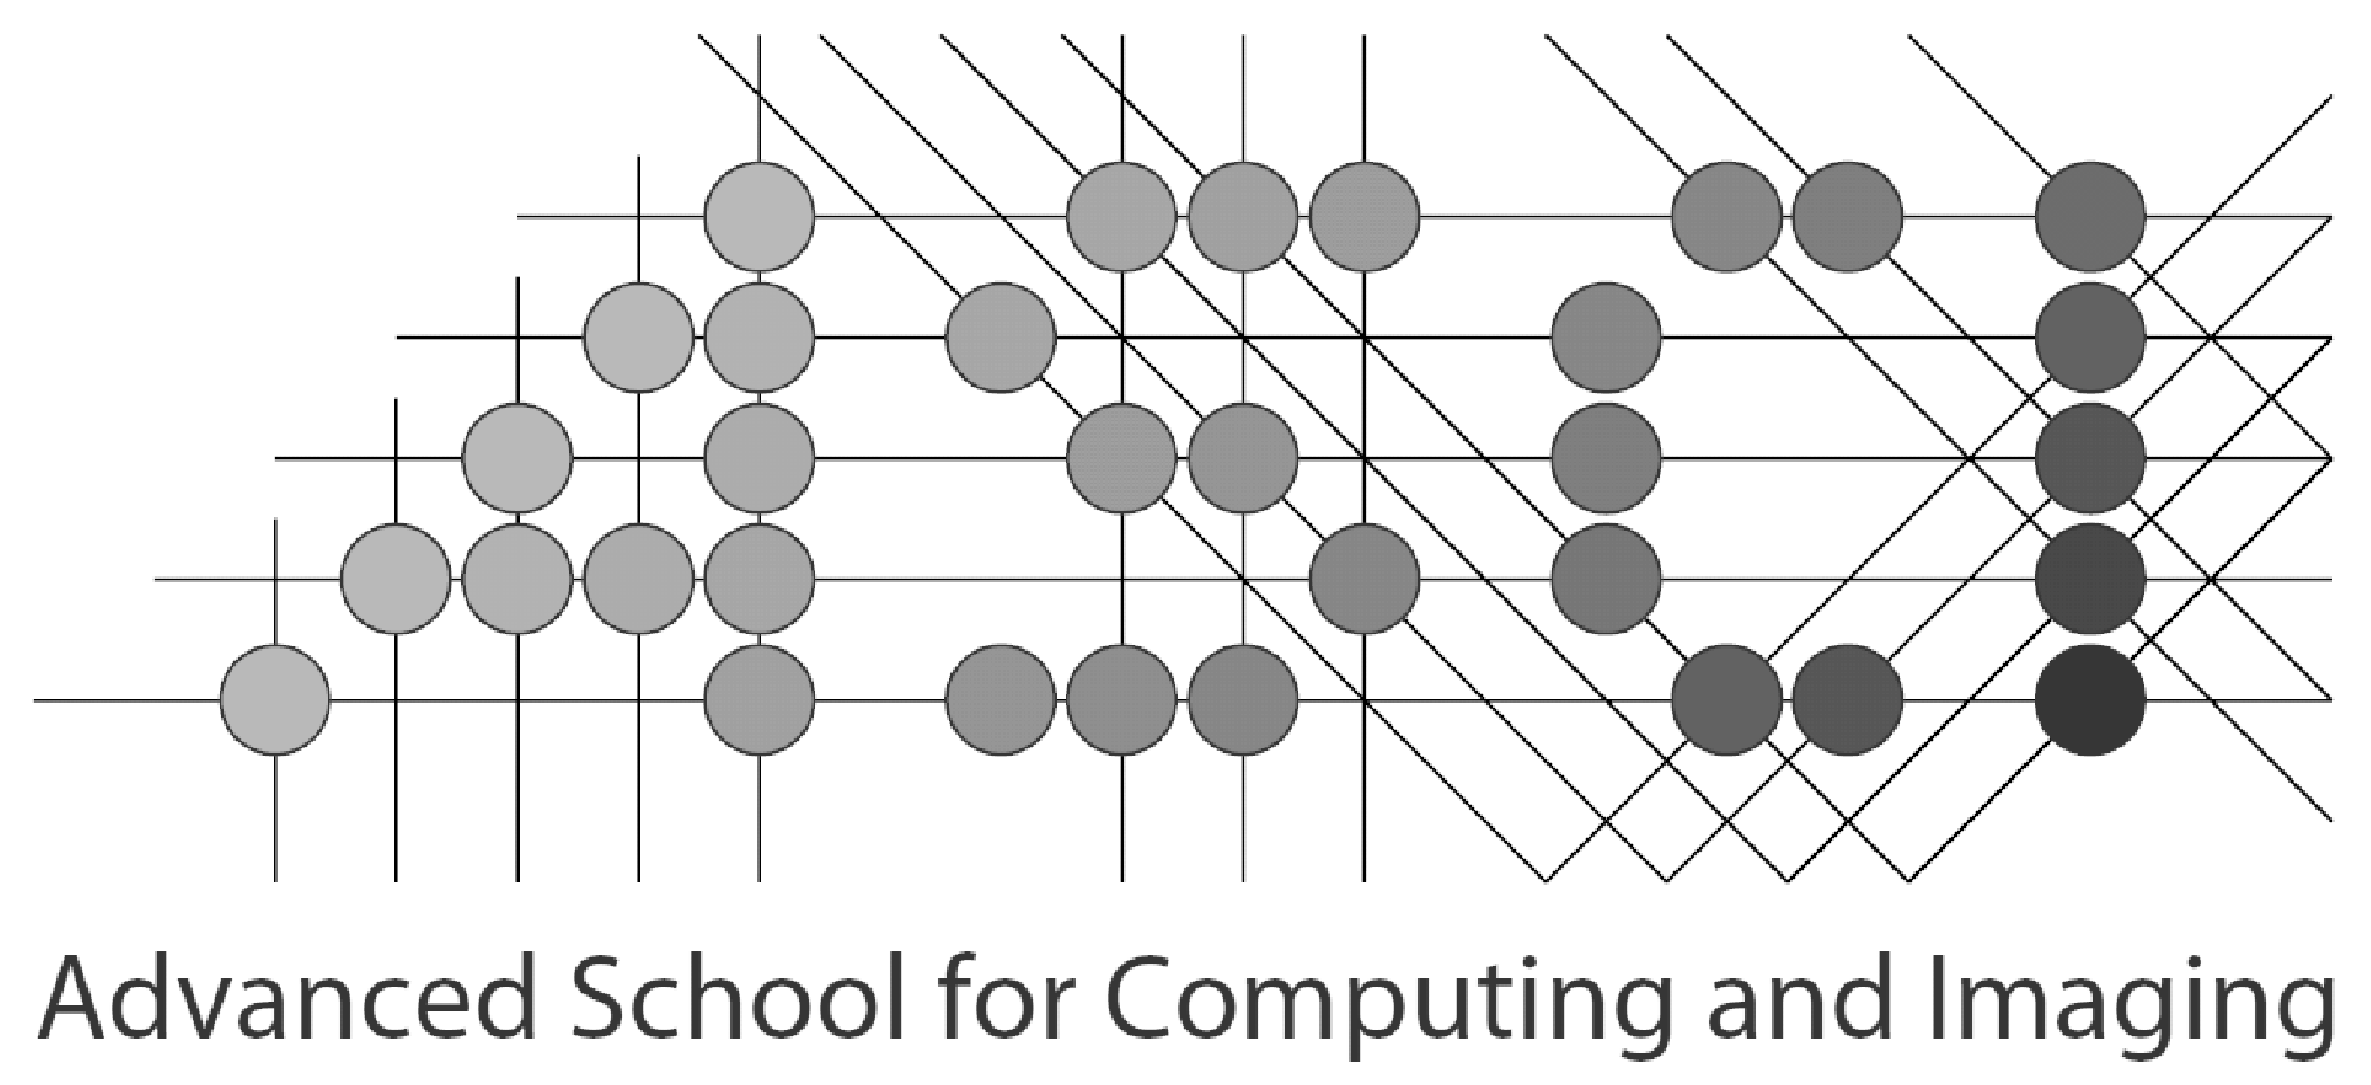
\includegraphics[height=15mm]{chapter_0/ASCIlogo-gray}
\hspace{100pt}
\includegraphics[height=15mm]{chapter_0/quva_logo}
\end{figure}


% table of contents
\tableofcontents
\markboth{Contents}{Contents}
\clearpage{\pagestyle{empty}\cleardoublepage}
\cleardoublepage

% chapters of the thesis
%!TEX root = thesis.tex

%%%%%%%%%%%%%%%%%%%%%%%%%%%%%%%%%%%%%%%%%%%
% Introduction
%%%%%%%%%%%%%%%%%%%%%%%%%%%%%%%%%%%%%%%%%%%
\chapter{Introduction}
\label{ch:intro}

% \section{Introduction}
\label{ch1:sec:intro}
%!TEX root = thesis.tex

Introduction
% \section{Method}
\label{ch1:sec:model}
%!TEX root = thesis.tex

Method
% \section{Related Work}
\label{ch1:sec:related}
%!TEX root = thesis.tex

Related Work
\section{List of Publications}
\label{ch1:sec:publications}
%!TEX root = thesis.tex

%%%%%%%%%%%%%%%%%%%%%%%%%%%%%%%%%%%%%%%%%%%
% 4. List of Publications
%%%%%%%%%%%%%%%%%%%%%%%%%%%%%%%%%%%%%%%%%%%

\begin{itemize}
\item
\textbf{Chapter~\ref{ch:unified-embedding}} is based on ``Unified Embedding and Metric Learning for Zero-Exemplar Event Detection", published in \textit{Computer Vision and Pattern Recognition (CVPR)}, 2017~\cite{hussein2017unified}, by Noureldien Hussein, Efstratios Gavves and Arnold W. M. Smeulders.
\vspace*{5pt}
\\
\textit{Contribution of authors}
\vspace*{5pt}
\\
Noureldien Hussein: all aspects,\\
Efstratios Gavves: guidance and technical advice,\\
Arnold W. M. Smeulders: supervision and insight.

\item
\textbf{Chapter~\ref{ch:timeception}} is based on ``TimeCeption for Complex Action Recognition", published in \textit{Computer Vision and Pattern Recognition (CVPR)}, 2019~\cite{hussein2017unified}, by Noureldien Hussein, Efstratios Gavves and Arnold W. M. Smeulders.
\vspace*{5pt}
\\
\textit{Contribution of authors}
\vspace*{5pt}
\\
Noureldien Hussein: all aspects,\\
Efstratios Gavves: guidance and technical advice,\\
Arnold W. M. Smeulders: supervision and insight.

\item
\textbf{Chapter~\ref{ch:videograph}} is based on ``VideoGraph: Recognizing Minutes-Long Human Activities in Videos", in submission to \textit{British Machine Vision Conference(BMVC)}, 2020~\cite{hussein2019videograph}, by Noureldien Hussein, Efstratios Gavves and Arnold W. M. Smeulders.
\vspace*{5pt}
\\
\textit{Contribution of authors}
\vspace*{5pt}
\\
Noureldien Hussein: all aspects,\\
Efstratios Gavves: guidance and technical advice,\\
Arnold W. M. Smeulders: supervision and insight.

\item
\textbf{Chapter~\ref{ch:pic}} is based on ``Permutation Invariant Convolution for Recognizing Long-range Activities", in submission to \textit{European Conference on Computer Vision (ECCV)}, 2019~\cite{hussein2017unified}, by Noureldien Hussein, Efstratios Gavves and Arnold W. M. Smeulders.
\vspace*{5pt}
\\
\textit{Contribution of authors}
\vspace*{5pt}
\\
Noureldien Hussein: all aspects,\\
Efstratios Gavves: guidance and technical advice,\\
Arnold W. M. Smeulders: supervision and insight.

\item
\textbf{Chapter~\ref{ch:timegate}} is based on ``TimeGate: Conditional Gating of Segments in Long-range Activities", in submission to \textit{European Conference on Computer Vision (ECCV)}, 2019~\cite{hussein2017unified}, by Noureldien Hussein, Mihir Jain and Babak Ehteshami Bejnordi.
\vspace*{5pt}
\\
\textit{Contribution of authors}
\vspace*{5pt}
\\
Noureldien Hussein: all aspects,\\
Mihir Jain: guidance and technical advice,\\
Babak Ehteshami Bejnordi: guidance and technical advice.

\end{itemize}

%%%%%%%%%%%%%%%%%%%%%%%%%%%%%%%%%%%%%%%%%%%
% Materials for the remaining chapters
%%%%%%%%%%%%%%%%%%%%%%%%%%%%%%%%%%%%%%%%%%%
% \section{Materials for the remaining chapters}

%!TEX root = thesis.tex

\chapter{Paper Name}
\label{ch:paper_name}

\todo{Add the content of your paper here}

\section{Introduction}
\label{ch2:sec:introduction}
%!TEX root = thesis.tex

\todo{Introduction}

\begin{figure}[!ht]
\begin{center}
\includegraphics[width=\linewidth]{example-image-golden}
\end{center}
\caption{Teaser figure.}
\label{ch2:fig:1-1}
\end{figure}
% \section{Related Work}
% \label{ch2:sec:related}
% \input{chapter_2/20_related_work}
% \section{Method}
% \label{ch2:sec:model}
% \input{chapter_2/30_method}
% \section{Experiments}
% \label{ch2:sec:experiments}
% \input{chapter_2/40_experiments}
% \section{Conclusion}
% \label{ch2:sec:conclusions}
% \input{chapter_2/50_conclusion}



%!TEX root = thesis.tex

\chapter{Conclusions}
\label{ch:conclusion}

\section{Summary}

Each paragraph has a summary of each chapter.
%!TEX root = thesis.tex

% %!TEX root = thesis.tex

\begin{appendices}

\chapter{Some Appendix}
The contents...

\section{This is section of appendix}

\end{appendices}
%!TEX root = thesis.tex

\chapter*{Samenvatting}
\addcontentsline{toc}{chapter}{Samenvatting}
\markboth{Samenvatting}{Samenvatting}

\section*{Thesis Title}

\todo Add Dutch Summary


%!TEX root = thesis.tex

\chapter*{Acknowledgments}
\addcontentsline{toc}{chapter}{Acknowledgments}

\todo Add Acknowledgments

% %!TEX root = thesis.tex

\chapter*{List of Publications}
\addcontentsline{toc}{chapter}{List of Publications}
\markboth{List of Publications}{List of Publications}


%\chapter*{Bibliography\markboth{Bibliography}{Bibliography}}
%\def\rightmark{Bibliography}

% \bibliography with small font
\cleardoublepage
\small
% \bibliographystyle{IEEEtrans}
\bibliographystyle{abbrv}
\footnotesize
\bibliography{thesis}
\addcontentsline{toc}{chapter}{Bibliography}
\small


\end{document}
